\documentclass{template}
\usepackage{graphicx}

\project{Comthings}
\title{AUT64 cryptanalyse}
\author{Kaci Amaouche}
\faculty{Arithmétique, codage et cryptologie}
\department{Mathématiques}
\setlength{\hoffset}{-18pt}        
\setlength{\oddsidemargin}{0pt} % Marge gauche sur pages impaires
\setlength{\evensidemargin}{9pt} % Marge gauche sur pages paires
\setlength{\marginparwidth}{54pt} % Largeur de note dans la marge
\setlength{\textwidth}{481pt} % Largeur de la zone de texte (17cm)
\setlength{\voffset}{-18pt} % Bon pour DOS
\setlength{\marginparsep}{7pt} % Séparation de la marge
\setlength{\topmargin}{0pt} % Pas de marge en haut
\setlength{\headheight}{13pt} % Haut de page
\setlength{\headsep}{10pt} % Entre le haut de page et le texte
\setlength{\footskip}{27pt} % Bas de page + séparation
\setlength{\textheight}{708pt} % Hauteur de la zone de texte (25cm)
\begin{document}
\chapter{Définition et présentation du système AUT64}

\section{Préliminaires}
\baselineskip=16pt
Nos conventions de notation sont les suivantes : lorsque nos opérandes sont des octets ou des quartets, nous utilisons les opérations $\land$, $\lor$, $\oplus$, $\ll$ et $\gg$ qui représentent respectivement les opérations logiques ET, OU, OU exclusif, décalage à gauche et décalage à droite. Nous utilisons $ \mathbin\Vert$ pour représenter la concaténation et nous utilisons le terme "symmetric byte" pour désigner un octet $b$ de la forme $n \mathbin\Vert n$ où $n \in F_{2}^{4}$. Lorsque nous décrivons des chaînes d'octets ou des tables de recherche, nous utilisons des crochets pour spécifier l'index. Nous utilisons les fonctions  $msb_m$ et $lsb_m$ qui renvoient respectivement les $m$ bits les plus significatifs et les moins significatifs. Lorsque notre opérande est un octet unique, nous utilisons les fonctions $un$ et $ln$ pour représenter $msb_4$ et $lsb_4$, respectivement. Lorsque $M$ est un ensemble, nous utilisons $m \overset{R}{\leftarrow} M$ pour désigner l'assignation à $m$ d'un élément de $M$ choisi uniformément au hasard.

$K$ est l'espace des clés, $M$ est l'espace des messages et $C$ est l'espace des textes chiffrés. Alors, un chiffrement par blocs est défini comme une paire d'algorithmes calculables efficacement, $E = (E, D),$ où $E : K \times M \to C$ et $D : K \times C \to M$, tel que pour tout $k \in K$, $M \in M$ :  $D(K, E(K, M)) = M$. 
    

\section{AUT64}
\baselineskip=16pt

Dans cette section, nous présentons tous les détails du chiffrement par blocs AUT64 et le protocole d'authentification de transpondeur TK5561 associé. La documentation publique sur AUT64 est rare. Le chiffrement est propriétaire et son code source est fermé, donc les seules informations largement disponibles proviennent d'une demande de brevet [BF03] et de la fiche technique du produit [TEM98]. Pour résoudre ce problème, nous avons procédé à l'ingénierie inverse complète du chiffrement par blocs AUT64 et de son implémentation, que nous publions ici en détail.

AUT64 a été identifié pour la première fois comme un chiffrement par blocs propriétaire utilisé dans la plupart des systèmes d'entrée sans clé du groupe Volkswagen entre environ 2004 et 2009 [GOKP16]. Dans cet article, nous présentons AUT64 tel qu'il est utilisé par le TK5561 d'Atmel, qui est un paquet de transpondeur automobile pour le circuit intégré d'identification cryptographique e5561 d'Atmel [TEM98]. L'e5561 utilise le chiffrement par blocs AUT64 et un protocole d'authentification propriétaire pour fournir une méthode d'authentification pour les systèmes d'immobilisation de véhicules. AUT64 est remarquable d'un point de vue de conception cryptographique car, en plus d'avoir une structure GUFN, sa clé symétrique de 120 bits définit une substitution et une permutation à partir desquelles les propriétés de sécurité du chiffrement sont dérivées.

Plus en détail, AUT64 est un chiffrement par blocs GUFN de 64 bits avec une taille de clé de 120 bits. Dans le TK5561, il comporte soit 8, soit 24 tours, en fonction de la configuration. L'espace de clés AUT64 est le triplet de toutes les chaînes binaires de 32 bits, de toutes les permutations à huit éléments et de toutes les permutations à seize éléments $K = (F_2^{32}, P_8, P_{16})$. La taille de clé de 120 bits correspond à la somme des 32, 24 et 64 bits occupés respectivement par les parties de clé $F_2^{32}$, $P_8$ et $P_{16}$. 
\subsubsection{Reverse Engineering AUT64}
\baselineskip=16pt
Nous avons effectué une rétro-ingénierie d'AUT64 à partir du système d'immobilisation "Module 142" de Mazda. Concrètement, nous avons récupéré le micrologiciel du microcontrôleur Motorola MC68HC05B6 utilisé dans cette boîte d'immobilisation à l'aide d'un programmeur standard. Ensuite, nous avons chargé le binaire du micrologiciel dans le désassembleur IDA Pro pour effectuer notre analyse. Nous avons pu localiser toutes les sous-routines cryptographiques importantes et reconstruire l'algorithme et le protocole AUT64. Nous avons mis en œuvre une version logicielle d'AUT64 et du protocole d'authentification en Python et en C pour développer, tester et évaluer nos attaques.

Nous avons vérifié nos résultats par rapport à la documentation disponible pour l'e5561 et une implémentation que nous avons créée pour les systèmes d'entrée sans clé à distance de VW [GOKP16]. Nous avons découvert que le système d'immobilisation utilise 24 tours d'AUT64 et le protocole d'authentification TK5561. Après avoir identifié AUT64 et le protocole d'authentification TK5561 dans le micrologiciel, nous avons pu localiser les parties de clé de permutation et de S-Box.

\begin{enumerate}
    \item La partie de clé de permutation $k_\sigma$ (page 6 dans la mémoire du transpondeur) est située dans les 32 premiers bits de la mémoire morte programmable (PROM) du microcontrôleur à partir de l'adresse 0x0800. Le $k_\sigma$ que nous avons récupéré est une permutation cyclique sans points fixes ;
    \item La partie de clé de substitution $k_\tau$ (page 8 et 7 dans la mémoire du transpondeur) est située dans les 64 bits qui suivent immédiatement la partie de clé de permutation. Elle est bijective, comme prévu, mais sinon sans particularité.
\end{enumerate}

Nous avons découvert que la clé de fonction de compression de 32 bits $k_G$ (page 5 dans la mémoire du transpondeur) n'est pas stockée dans la boîte d'immobilisation du véhicule. Au lieu de cela, la station de base calcule $k_G$ en fonction de l'ID du transpondeur (IDcode) qui est transmis au début du protocole d'authentification.
\subsubsection{Chiffrement}
\baselineskip=16pt
La figure suivante présente le fonctionnement d'AUT64.
\begin{figure}
    \centering
    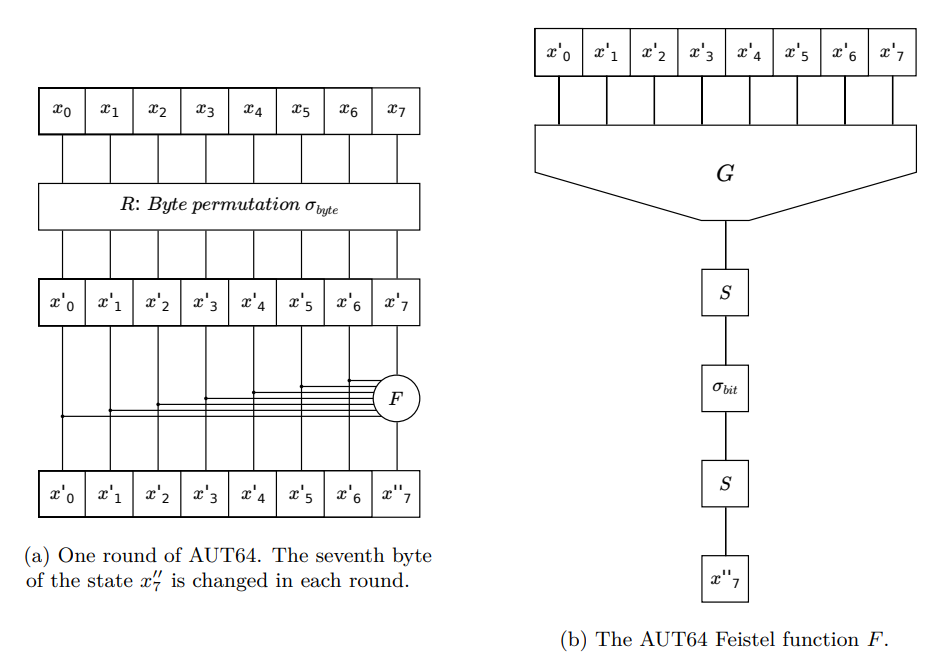
\includegraphics[width=\textwidth]{Cipher.PNG}
    \caption{AUT64 structure algorithmique}
    \label{fig:image}
\end{figure}

\textbf{Définition 1  (État du chiffrement AUT64)} Nous définissons un état du chiffrement AUT64, noté $X$, comme un élément de $F_{64}^2$ où $X$ est composé de huit octets $x_0, ..., x_7$, chacun étant un élément de $F_{8}^2$.

AUT64 est un GUFN (Réseau de Feistel généralisé) où le bloc source est l'état du chiffrement $X$ et le bloc cible est l'octet $x_7 \in X$.

La permutation d'octets $R$ et la fonction Feistel $F$ dépendent toutes deux de la clé.

\textbf{Définition 2 (Spécification de la clé AUT64)} : Nous définissons une clé AUT64 comme un triplet $K \in \langle kG, k\sigma, k\tau \rangle$ où :

\begin{enumerate}
  \item $kG \in F_{32}^2$ est un mot de 32 bits à partir duquel les clés de chaque tour sont dérivées ;
  \item $k\sigma$ est une permutation à 8 éléments qui définit à la fois la permutation de byte $\sigma_{\text{byte}}$ et la permutation de bit $\sigma_{\text{bit}}$ de la fonction Feistel ;
  \item $k\tau$ est une permutation à 16 éléments qui définit la S-Box $\tau$ de taille 4x4 bijective dans la fonction Feistel.
\end{enumerate}
Chaque tour d'AUT64 comprend deux composants :
\begin{enumerate}
    \item Une permutation de byte $R(X) = X_0$ où $R(x_0 \ldots x_7) = \begin{pmatrix} \sigma_{\text{byte}}(X)[0] \\ \vdots \\ \sigma_{\text{byte}}(X)[7] \end{pmatrix}$
    \item Une fonction de Feistel $F(X_0) = x_{7}^{"}$.
\end{enumerate}

Dans chaque tour d'AUT64, l'état est permuté par $R : X \rightarrow X^{'}$, puis la fonction de Feistel est appliquée par $F : X^{'} \rightarrow X^{"}$. La structure d'AUT64 nécessite qu'un bit de l'état apparaisse à la fois dans les blocs source et cible, cela doit donc être appliqué pendant un minimum de huit tours. On peut donc en déduire que la permutation de byte doit avoir une longueur de cycle de huit. Si la permutation avait des points fixes, alors les bits du texte en clair resteraient inchangés dans le texte chiffré. Dans le reste de ce document, nous supposons que l'algorithme de génération de clé choisit effectivement des permutations avec une longueur de cycle de huit.

Le brevet TK5561 [BF03] spécifie une procédure de génération de clé qui s'aligne avec la manière dont la clé AUT64 est composée. Il y a trois parties :
\begin{enumerate} 
    \item La partie de clé de fonction de compression $k_G$ est une chaîne de bits aléatoire générée à l'aide du chiffrement de bloc DES qui est initialisée par le fabricant automobile. Aucune autre information n'est donnée dans le brevet ;
    \item La partie de clé de permutation $kσ$ est appelée "clé de famille". Chaque fabricant automobile se voit attribuer douze bits, puis choisit parmi seize possibilités pour les douze bits restants ;
    \item La partie de clé de substitution $kτ$ est appelée "clé utilisateur". La clé est générée à l'aide d'une méthode propriétaire non spécifiée. Le brevet affirme qu'une répétition ne se produira qu'après la génération de $20,9 \times  10^{12}$ clés utilisateur. Nous pouvons en conclure que l'ensemble complet de S-Box $4\times 4$ est utilisé.   
\end{enumerate} 

\textbf{Définition 3} (Fonction de Feistel AUT64): La fonction de Feistel AUT64, F, est construite à partir des quatre composants suivants :
\begin{enumerate}
    \item Une fonction de compression $G(X^{'}) = g$ qui mappe un état d'entrée permuté $X^{'} \in F_2^{64}$ vers un byte de sortie $g \in F_2^{8}$ ;
    \item Une opération de substitution  $S(g) = \tau(\text{un}(g)) \, || \, \tau(\text{ln}(g))$
 qui consiste en deux S-Box 4×4 identiques $\tau$  appliqués indépendamment aux moitiés supérieures et inférieures du byte g ;
    \item Une opération de permutation $\sigma_{\text{bit}}(S(g))$ qui applique la même transposition que $\sigma_{\text{byte}}$ mais au niveau des bits sur la sortie de S(g) ;
    \item L'opération de substitution appliquée à la sortie de l'opération de permutation par bits, $x_7^{"} = S(\sigma_{\text{bit}}(S(g)))$.
\end{enumerate}
Les trois dernières opérations forment un réseau de substitution-permutation (SPN).


\textbf{Définition 4} (Définition des clés de tour d'AUT64) : Lorsque r est le numéro du tour et i l'index du byte dans l'état de tour permuté X0, nous définissons


$u_k(k_G, r, i) = k_G[\text{$T_U$}[(r \times 8) + i]]$

 
$l_k(k_G, r, i) = k_G[\text{$T_L$}[(r \times 8) + i]]$

 qui renvoie le nibble de clé de tour inférieur et supérieur, respectivement.

 La figure suivante montre le fonctionnement de la fonction de compression $G$

 \begin{figure}
    \centering
    \includegraphics[width=\textwidth]{Compression.PNG}
    \caption{AUT64-Fonction de compression $G$}
    \label{fig:image}
\end{figure}


\textbf{Définition 6}  (Fonction de compression AUT64) La fonction de compression AUT64, notée $G$, prend en entrée la partie de clé $k_G$, l'état de bloc permuté $X^{'}$ et le numéro de tour $r$. $G$ produit la concaténation de deux variables internes calculées comme suit :


$gl = \sum_{i=0}^{7} \text{T}_{\text{offset}}[l_k(k_G, r, i)] \, || \, ln(X_i^{'})$

$gu = \sum_{i=0}^{7} \text{T}_{\text{offset}}[l_k(k_G, r, i)] \, || \, un(X_i^{'})$

\subsubsection{Protocole d'authentification}
\baselineskip=16pt
\textbf{Définition 7} (Authentification AUT64) :

Nous définissons l'authentification AUT64 comme le quartet d'algorithmes $A = (\text{EncAUT64}, C, R, H)$, où pour toutes les clés AUT64 $K \in \langle k_G, k_\sigma, k_\tau \rangle$, pour tous les sommes de contrôle $h \in F_2^{5}$ et pour toutes les nonces et les défis $(X, Y) \in F_{64}^2$ :

\begin{itemize}
    \item \textbf{EncAUT64} : $X \mapsto \text{EncAUT64}(K, X)$ est l'algorithme de chiffrement AUT64.
    \item \textbf{C} : $Y \mapsto C(k_G, X)$ est l'algorithme de défi du protocole, qui est clé avec la partie clé de la fonction de compression $k_G \in K$.
    \item \textbf{R} : $X \mapsto R(k_G, Y)$ est l'algorithme de récupération de nonce du protocole, qui est clé avec $k_G$ et calcule l'image antérieure de $C_k_G$ telle que $\forall k_G \in F_{32}^2$ et $\forall X \in F_{64}^2$, l'équation de cohérence suivante est satisfaite : $X = R_{k_G}(C_{k_G}(X))$.
    \item \textbf{H} : $h \mapsto H(Y)$ calcule le poids de Hamming de $Y$.
\end{itemize}

 \begin{figure}
    \centering
    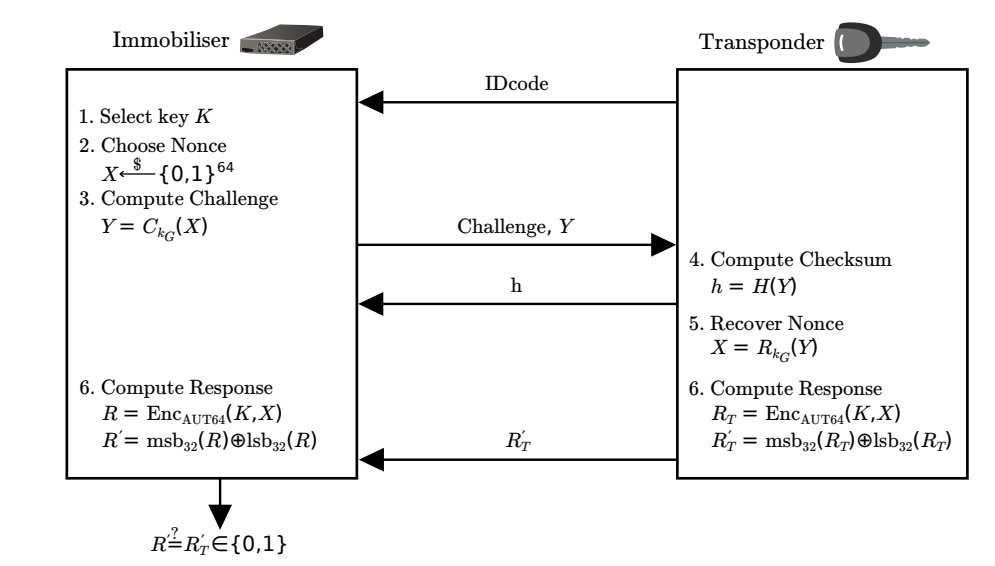
\includegraphics[width=\textwidth]{auth.PNG}
    \caption{AUT64-authentification}
    \label{fig:image}
\end{figure}


\chapter{Cryptanalyse d'AUT64}
\section{La taille réelle de la clé}
Comme mentionné précédemment, la clé secrète est constituée de 3 clés, à savoir $K \in \langle k_G, k_\sigma, k_\tau \rangle$.

\begin{itemize}
    \item La clé $k_G$ est une clé de 32 bits. Les auteurs ont démontré qu'en établissant simplement une connexion avec le transpondeur, il est possible de reconstituer la clé $k_G$ selon la procédure suivante :
    
Soit $ID0_$, $ID_1$, $ID_2$ et $ID_3$ les 4 octets qui composent le code d'identification du transpondeur, et soit $u = (ID_0 \land 0xE) \ll 1$. En utilisant la table de recherche de dérivation de clé ($T_D$) figurant dans l'Annexe A, chaque octet de $k_G$ est dérivé comme suit : 
    
    \begin{align*}
        k_G_0 &= ID_0 \oplus T_D[u] \oplus k_G_3 \\
        k_G_1 &= ID_1 \oplus T_D[1 + u] \oplus k_G_3 \\
        k_G_2 &= ID_2 \oplus T_D[2 + u] \oplus k_G_3 \\
        k_G_3 &= ID_3 \oplus T_D[3 + u]
    \end{align*}
\end{itemize}

\begin{itemize}
    \item La clé $k_\sigma$ est définie comme étant une clé de 24 bits (8$\times$3), que l'on peut visualiser comme un tableau de 8 éléments, où chaque élément est constitué de 3 bits. Cependant, en réalité, sa taille effective n'est pas de 24 bits, car c'est une clé de permutation. Ainsi, elle aura une taille d'environ $8!$ ce qui est presque équivalent à 15.3 bits. Les auteurs ont démontré que la permutation est cyclique, ce qui signifie qu'elle n'a que $(8-1)!$, soit environ 12.3 bits.
\end{itemize}


\begin{itemize}
    \item La clé $k_\tau$ est une S-box de dimension 4$\times$4, ce qui signifie qu'elle est constituée de 16 éléments. Chaque élément de la S-box est représenté sur 4 bits. En raison de ses propriétés en tant que S-box, sa taille effective est de $16!$ ce qui équivaut à environ 44.3 bits

\end{itemize}

La taille réelle de la clé n'est pas de $120$ bits, mais plutôt de $32 + 12.3 + 44.3 = 88.6$ bits
\section{Attaque théorique}
\baselineskip=16pt

Les auteurs ont démontré qu'il était possible de casser ce système en quelques secondes pour les 8 tours. Cependant, cette démonstration suppose un scénario spécifique impliquant un attaquant A et l'oracle du système AUT64. Dans ce scénario, l'attaquant envoie des plaintexts soigneusement choisis au système, récupère les chiffrés correspondants, puis utilise des techniques d'analyse cryptographique pour reconstituer les 2 clés restantes.

Il est important de noter que ce scénario est une attaque à plaintext choisis, ce qui signifie que l'attaquant a un contrôle total sur les plaintexts utilisés pour le chiffrement. De plus, cette attaque nécessite une grande quantité de paires clair/chiffré, ce qui la rend difficilement réalisable dans la vraie vie.

Il est donc essentiel de considérer le contexte et les conditions spécifiques de cette démonstration. Dans un environnement réel, les conditions peuvent être différentes, et la sécurité du système AUT64 pourrait être plus robuste face à d'autres types d'attaques ou de scénarios d'utilisation.

\section{Attaque réelle}
\baselineskip=16pt

Dans une attaque pratique, en particulier contre AUT64 avec 24 tours, la reconstitution des 3 clés n'est pas particulièrement complexe. Voici comment chaque clé peut être reconstituée :

\begin{itemize}
    \item Pour la clé $k_G$, comme mentionné précédemment, il est possible de la reconstituer en établissant simplement une connexion avec le transpondeur, ce qui rend cette opération instantanée.
    
    \item Pour la clé de permutation $k_\sigma$ , les auteurs ont démontré que le schéma de gestion de clé AUT64 réduit l'espace des clés de permutation à seulement 16 clés par fabricant de véhicules. Cela signifie qu'en lisant $k_\sigma$ à partir de deux unités d'immobilisation différentes et en identifiant la partie constante, l'espace des clés $k_\sigma$ d'AUT64 n'est plus que de 2.6 bits. 
    
    \item Pour la clé $k_\tau$, comme mentionné précédemment, étant une S-box à 16 éléments, elle a une taille de seulement $16!$, ce qui équivaut à environ $44.3$ bits.
\end{itemize}

Une fois que la clé $k_\sigma$ est connue, l'espace des clés n'est plus que de $16!$ =  $2^{44.3}$ et peut être trouvé en quelques minutes en utilisant une recherche exhaustive avec des instances parallèles basées sur GPU d'Amazon EC2. 

Il est important de noter que la sécurité d'un système cryptographique dépend de la complexité de reconstitution de ses clés. Dans le cas d'AUT64, certaines clés peuvent être récupérées relativement facilement, ce qui soulève des inquiétudes concernant la robustesse de ce système. Des mesures de sécurité supplémentaires peuvent être nécessaires pour renforcer la résistance de ce système face aux attaques.

\section{En résumé...}
\baselineskip=16pt

En pratique, pour pouvoir compromettre le système, il existe deux approches possibles :
\begin{itemize}
    \item Première solution : Les chercheurs qui ont examiné ce système ont identifié des indices suggérant que le système en question utilise effectivement des constantes $k_\tau$ et $k_\sigma$ pour un ensemble de véhicules. Plus précisément, ils ont récupéré ces constantes $k_\sigma$ et $k_\tau$ à partir de deux boîtiers d'immobilisation différents et ont obtenu des valeurs identiques. Si cette supposition peut être vérifiée, cela signifie que la clé complète du transpondeur peut être récupérée en se basant uniquement sur la connaissance du code ID (pour calculer $k_G$) ainsi que sur les valeurs propres au fabricant $k_\sigma$ et $k_\tau$, sans nécessiter d'autres analyses cryptographiques supplémentaires. En conséquence, il suffirait de récupérer ces trois variables pour reconstituer instantanément la clé.
    
    \item Deuxième solution : Les systèmes d'immobilisation étudiés utilisent AUT64 dans sa configuration à 24 tours. Pour récupérer $k_\sigma$ et $k_\tau$, nous commençons par obtenir $K_G$ en fonction de la capture du code ID du transpondeur (une liste de clés est donnée en dessous). La taille de clé anticipée restante est $|K| = 16! \times 7! \approx 2^{56.5}$ (en supposant que toutes les permutations cycliques et toutes les boîtes S 4x4 sont possibles), ce qui se situe déjà dans la plage des dispositifs de force brute. Cependant, une propriété du schéma de gestion de clé spécifié dans le brevet AUT64 est qu'il ne laisse que seize clés de permutation possibles (la soi-disant "clé de famille") par fabricant de véhicules. Cela signifie qu'en lisant $k_\sigma$ à partir de deux boîtiers d'immobilisation différents et en identifiant la partie constante (et cela en pourra le faire en analysant des firmwares), l'espace de clé restant d'AUT64 est seulement $|K| = 16! \times 16 \approx 2^{48.3}$
    Et enfin, pour pouvoir vérifier la validité de la clé récupérée, il nous faut un plaintext qu'on va chiffrer avec cette  clé candidate et le comparer avec le ciphertext capturé.

\section{Liste des clés}
\baselineskip=16pt


\end{itemize}
\begin{enumerate}
  \item Clé À Transpondeur D'Origine Mazda 626 Mpv Mx5 Bjyv-76-2Gx 8C Maz13
  \begin{itemize}
    \item \href{https://abkeys.com/fr/collections/transponder-keys-cloning-keys/products/mazda-626-miata-mpv-transponder-key-8c-chip-maz13-bjyv-76-2gx-1826}{lien}
  \end{itemize}
  
   \item Clé Mazda Premacy 1999–2004
  \begin{itemize}
    \item \href{https://www.cle-de-voiture-paris.fr/cle-mazda-premacy-1999-2004/}{lien}
  \end{itemize}
  
  \item Clé Mazda MPV 1999–2006 
  \begin{itemize}
    \item \href{https://www.cle-de-voiture-paris.fr/cle-mazda-mpv-1999-2006/}{lien} 
  \end{itemize}
  
   \item CLE FORD RANGER MAZDA PREMACY PROTON 415 416
  \begin{itemize}
    \item \href{https://srotas.fr/product/s27555036720/}{lien}
  \end{itemize}
\end{enumerate}
\end{enumerate}
\chapter{Références}
1-Dismantling the AUT64 Automotive Cipher :

\textit{Christopher Hicks, Flavio D. Garcia and David Oswald} 
\url{https://tches.iacr.org/index.php/TCHES/article/view/874/826}.\\



2-Cryptographic Key Management for the Vehicles of Tomorrow :

\textit{Christopher Richard Allden Hicks} \url{https://etheses.bham.ac.uk//id/eprint/10442/1/Hicks2020PhD.pdf}.\\
\end{document}
